% Options for packages loaded elsewhere
\PassOptionsToPackage{unicode}{hyperref}
\PassOptionsToPackage{hyphens}{url}
%
\documentclass[
  ignorenonframetext,
]{beamer}
\usepackage{pgfpages}
\setbeamertemplate{caption}[numbered]
\setbeamertemplate{caption label separator}{: }
\setbeamercolor{caption name}{fg=normal text.fg}
\beamertemplatenavigationsymbolsempty
% Prevent slide breaks in the middle of a paragraph
\widowpenalties 1 10000
\raggedbottom
\setbeamertemplate{part page}{
  \centering
  \begin{beamercolorbox}[sep=16pt,center]{part title}
    \usebeamerfont{part title}\insertpart\par
  \end{beamercolorbox}
}
\setbeamertemplate{section page}{
  \centering
  \begin{beamercolorbox}[sep=12pt,center]{part title}
    \usebeamerfont{section title}\insertsection\par
  \end{beamercolorbox}
}
\setbeamertemplate{subsection page}{
  \centering
  \begin{beamercolorbox}[sep=8pt,center]{part title}
    \usebeamerfont{subsection title}\insertsubsection\par
  \end{beamercolorbox}
}
\AtBeginPart{
  \frame{\partpage}
}
\AtBeginSection{
  \ifbibliography
  \else
    \frame{\sectionpage}
  \fi
}
\AtBeginSubsection{
  \frame{\subsectionpage}
}
\usepackage{amsmath,amssymb}
\usepackage{lmodern}
\usepackage{ifxetex,ifluatex}
\ifnum 0\ifxetex 1\fi\ifluatex 1\fi=0 % if pdftex
  \usepackage[T1]{fontenc}
  \usepackage[utf8]{inputenc}
  \usepackage{textcomp} % provide euro and other symbols
\else % if luatex or xetex
  \usepackage{unicode-math}
  \defaultfontfeatures{Scale=MatchLowercase}
  \defaultfontfeatures[\rmfamily]{Ligatures=TeX,Scale=1}
  \setmainfont[BoldFont = SF Pro Rounded Semibold]{SF Pro Rounded}
  \setmathfont[]{STIX Two Math}
\fi
\usefonttheme{serif} % use mainfont rather than sansfont for slide text
% Use upquote if available, for straight quotes in verbatim environments
\IfFileExists{upquote.sty}{\usepackage{upquote}}{}
\IfFileExists{microtype.sty}{% use microtype if available
  \usepackage[]{microtype}
  \UseMicrotypeSet[protrusion]{basicmath} % disable protrusion for tt fonts
}{}
\makeatletter
\@ifundefined{KOMAClassName}{% if non-KOMA class
  \IfFileExists{parskip.sty}{%
    \usepackage{parskip}
  }{% else
    \setlength{\parindent}{0pt}
    \setlength{\parskip}{6pt plus 2pt minus 1pt}}
}{% if KOMA class
  \KOMAoptions{parskip=half}}
\makeatother
\usepackage{xcolor}
\IfFileExists{xurl.sty}{\usepackage{xurl}}{} % add URL line breaks if available
\IfFileExists{bookmark.sty}{\usepackage{bookmark}}{\usepackage{hyperref}}
\hypersetup{
  pdftitle={305 Lecture 11.5 - Example Models},
  pdfauthor={Brian Weatherson},
  hidelinks,
  pdfcreator={LaTeX via pandoc}}
\urlstyle{same} % disable monospaced font for URLs
\newif\ifbibliography
\setlength{\emergencystretch}{3em} % prevent overfull lines
\providecommand{\tightlist}{%
  \setlength{\itemsep}{0pt}\setlength{\parskip}{0pt}}
\setcounter{secnumdepth}{-\maxdimen} % remove section numbering
\let\Tiny=\tiny

 \setbeamertemplate{navigation symbols}{} 

% \usetheme{Madrid}
 \usetheme[numbering=none, progressbar=foot]{metropolis}
 \usecolortheme{wolverine}
 \usepackage{color}
 \usepackage{MnSymbol}
% \usepackage{movie15}

\usepackage{amssymb}% http://ctan.org/pkg/amssymb
\usepackage{pifont}% http://ctan.org/pkg/pifont
\newcommand{\cmark}{\ding{51}}%
\newcommand{\xmark}{\ding{55}}%

\DeclareSymbolFont{symbolsC}{U}{txsyc}{m}{n}
\DeclareMathSymbol{\boxright}{\mathrel}{symbolsC}{128}
\DeclareMathAlphabet{\mathpzc}{OT1}{pzc}{m}{it}

\usepackage{tikz-qtree}
% \usepackage{markdown}
%\RequirePackage{bussproofs}
\usetikzlibrary{arrows.meta}
\RequirePackage[tableaux]{prooftrees}
\forestset{line numbering, close with = x}
% Allow for easy commas inside trees
\renewcommand{\,}{\text{, }}


\usepackage{tabulary}

\usepackage{open-logic-config}

\setlength{\parskip}{1ex plus 0.5ex minus 0.2ex}

\AtBeginSection[]
{
\begin{frame}
	\Huge{\color{darkblue} \insertsection}
\end{frame}
}

\renewenvironment*{quote}	
	{\list{}{\rightmargin   \leftmargin} \item } 	
	{\endlist }

\definecolor{darkgreen}{rgb}{0,0.7,0}
\definecolor{darkblue}{rgb}{0,0,0.8}

\newcommand{\starttab}{\begin{center}
\vspace{6pt}
\begin{tabular}}

\newcommand{\stoptab}{\end{tabular}
\vspace{6pt}
\end{center}
\noindent}


\newcommand{\sif}{\rightarrow}
\newcommand{\siff}{\leftrightarrow}
\newcommand{\EF}{\end{frame}}


\newcommand{\TreeStart}[1]{
%\end{frame}
\begin{frame}
\begin{center}
\begin{tikzpicture}[scale=#1]
\tikzset{every tree node/.style={align=center,anchor=north}}
%\Tree
}

\newcommand{\TreeEnd}{
\end{tikzpicture}
%\end{center}
}

\newcommand{\DisplayArg}[2]{
\begin{enumerate}
{#1}
\end{enumerate}
\vspace{-6pt}
\hrulefill

%\hspace{14pt} #2
%{\addtolength{\leftskip}{14pt} #2}
\begin{quote}
{\normalfont #2}
\end{quote}
\vspace{12pt}
}

\newenvironment{ProofTree}[1][1]{
\begin{center}
\begin{tikzpicture}[scale=#1]
\tikzset{every tree node/.style={align=center,anchor=south}}
}
{
\end{tikzpicture}
\end{center}
}

\newcommand{\TreeFrame}[2]{
\begin{columns}[c]
\column{0.5\textwidth}
\begin{center}
\begin{prooftree}{}
#1
\end{prooftree}
\end{center}
\column{0.45\textwidth}
%\begin{markdown}
#2
%\end{markdown}
\end{columns}
}

\newcommand{\ScaledTreeFrame}[3]{
\begin{columns}[c]
\column{0.5\textwidth}
\begin{center}
\scalebox{#1}{
\begin{prooftree}{}
#2
\end{prooftree}
}
\end{center}
\column{0.45\textwidth}
%\begin{markdown}
#3
%\end{markdown}
\end{columns}
}

\usepackage[bb=boondox]{mathalfa}
\DeclareMathAlphabet{\mathbx}{U}{BOONDOX-ds}{m}{n}
\SetMathAlphabet{\mathbx}{bold}{U}{BOONDOX-ds}{b}{n}
\DeclareMathAlphabet{\mathbbx} {U}{BOONDOX-ds}{b}{n}


\newenvironment{oltableau}{\center\tableau{}} %wff format={anchor = base west}}}
       {\endtableau\endcenter}
       
\newcommand{\formula}[1]{$#1$}

\usepackage{tabulary}
\usepackage{booktabs}

\def\begincols{\begin{columns}}
\def\begincol{\begin{column}}
\def\endcol{\end{column}}
\def\endcols{\end{columns}}

\usepackage[italic]{mathastext}
\usepackage{nicefrac}

\definecolor{mygreen}{RGB}{0, 100, 0}
\definecolor{mypink2}{RGB}{219, 48, 122}
\definecolor{dodgerblue}{RGB}{30,144,255}

%\def\True{\textcolor{dodgerblue}{\text{T}}}
%\def\False{\textcolor{red}{\text{F}}}

\def\True{\mathbb{T}}
\def\False{\mathbb{F}}

% This is because arguments didn't have enough space after them
\usepackage{etoolbox}
\AfterEndEnvironment{description}{\vspace{9pt}}
\AfterEndEnvironment{oltableau}{\vspace{9pt}}
\BeforeBeginEnvironment{oltableau}{\vspace{9pt}}
\AfterEndEnvironment{center}{\vspace{12pt}}
\BeforeBeginEnvironment{tabular}{\vspace{9pt}}

\setlength\heavyrulewidth{0pt}
\setlength\lightrulewidth{0pt}

%\def\toprule{}
%\def\bottomrule{}
%\def\midrule{}

\setbeamertemplate{caption}{\raggedright\insertcaption}

\usepackage{tikz}
%\usepackage{amsmath, amssymb}
\usetikzlibrary{positioning,arrows,calc}

\tikzset{
  modal/.style={>=stealth',
    shorten >=1pt,
    shorten <=1pt,
    auto,
    node distance=1.5cm,
    label distance=2pt,
    semithick},
  every label/.style={phantom,align=left},
  world/.style = {circle,draw,minimum size=0.5cm,fill=gray!15},
  modal every node/.style={world},
  point/.style={circle,draw,inner sep=0.5mm,fill=black},
  phantom/.style={rectangle,inner sep=0pt,draw=none,fill=none},
  reflexive above/.style={->,loop,looseness=7,in=60,out=120},
  reflexive below/.style={->,loop,looseness=7,in=240,out=300},
  reflexive left/.style={->,loop,looseness=7,in=150,out=210},
  reflexive right/.style={->,loop,looseness=7,in=30,out=330}
}
\ifluatex
  \usepackage{selnolig}  % disable illegal ligatures
\fi

\title{305 Lecture 11.5 - Example Models}
\author{Brian Weatherson}
\date{}

\begin{document}
\frame{\titlepage}

\begin{frame}{Plan}
\protect\hypertarget{plan}{}
\begin{itemize}
\tightlist
\item
  To illustrate what we've done so far with some worked examples.
\end{itemize}
\end{frame}

\begin{frame}{Associated Reading}
\protect\hypertarget{associated-reading}{}
\begin{itemize}
\tightlist
\item
  Boxes and Diamonds, section 3.6 and 3.7.
\end{itemize}
\end{frame}

\begin{frame}
I'm going to go through the table on page 49 of the textbook, and show
how there can be models where each of them is false. And I'll add a
couple more in besides. \pause Here is what we'll cover

\begin{enumerate}
\tightlist
\item
  \(\Box(A \vee B) \rightarrow (\Box A \vee \Box B)\)
\item
  \((\Diamond A \wedge \Diamond B) \rightarrow \Diamond (A \wedge B)\)
\item
  \(A \rightarrow \Box A\)
\item
  \(\Box A \rightarrow A\)
\item
  \(\Box \Diamond A \rightarrow B\)
\item
  \(\Box \Diamond A \rightarrow A\)
\item
  \(\Box \Box A \rightarrow \Box A\)
\item
  \(\Box A \rightarrow \Box \Box A\)
\item
  \(\Box \Diamond A \rightarrow \Diamond \Box A\)
\item
  \(\Box A \rightarrow \Diamond A\)
\end{enumerate}
\end{frame}

\begin{frame}{\(\Box(A \vee B) \rightarrow (\Box A \vee \Box B)\)}
\protect\hypertarget{boxa-vee-b-rightarrow-box-a-vee-box-b}{}
\begin{columns}
    \begin{column}{0.65\textwidth}
        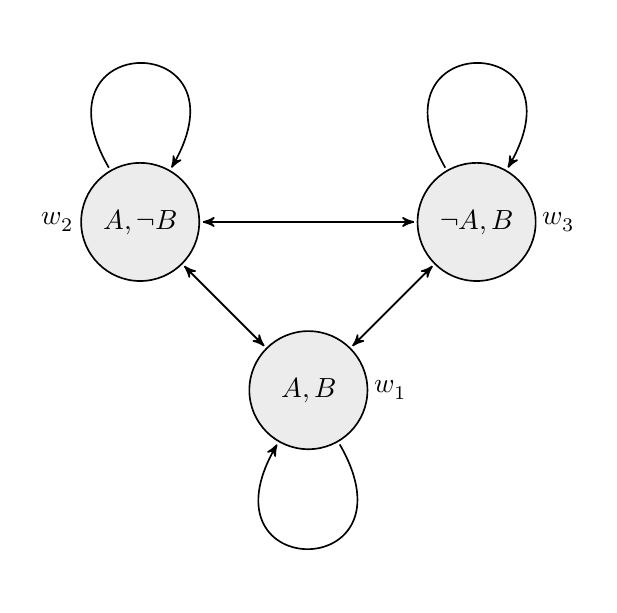
\begin{tikzpicture}[scale=0.6,modal,world/.append style={minimum size=1.5cm}]
      \node[world] (w1) [label=right:$w_1$]{$A,B$}; 
      \node[world] (w2) [label=left:$w_2$, above left=of w1]{$A, \neg B$}; 
      \node[world] (w3) [label=right:$w_3$, above right=of w1] {$\neg A, B$};
      \draw[->] (w1) to (w2);
      \draw[->] (w1) to (w3);
      \draw[->] (w2) to (w1);
      \draw[->] (w3) to (w1);
      \draw[->] (w3) to (w2);
      \draw[->] (w2) to (w3);
      \path[->] (w2) edge[reflexive above] (w2);
      \path[->] (w3) edge[reflexive above] (w3);
      \path[->] (w1) edge[reflexive below] (w1);
    \end{tikzpicture}
    \end{column}
    \begin{column}{0.3\textwidth}
At all points, either $A$ or $B$ is true, so $\Box(A \vee B)$ is true. \pause 

\bigskip

But $\Box A$ and $\Box B$ are false everywhere. \pause So the conditional is false everywhere.
\end{column}
\end{columns}
\end{frame}

\begin{frame}{\(\Box(A \vee B) \rightarrow (\Box A \vee \Box B)\)}
\protect\hypertarget{boxa-vee-b-rightarrow-box-a-vee-box-b-1}{}
\begin{columns}
    \begin{column}{0.65\textwidth}
        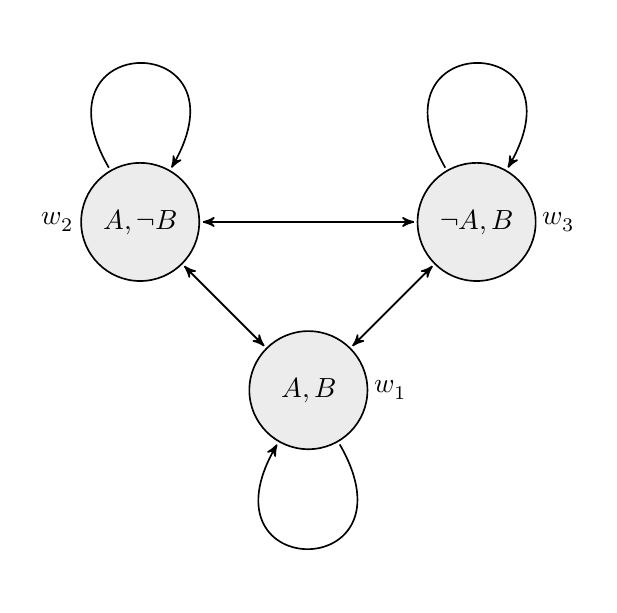
\begin{tikzpicture}[scale=0.6,modal,world/.append style={minimum size=1.5cm}]
      \node[world] (w1) [label=right:$w_1$]{$A,B$}; 
      \node[world] (w2) [label=left:$w_2$, above left=of w1]{$A, \neg B$}; 
      \node[world] (w3) [label=right:$w_3$, above right=of w1] {$\neg A, B$};
      \draw[->] (w1) to (w2);
      \draw[->] (w1) to (w3);
      \draw[->] (w2) to (w1);
      \draw[->] (w3) to (w1);
      \draw[->] (w3) to (w2);
      \draw[->] (w2) to (w3);
      \path[->] (w2) edge[reflexive above] (w2);
      \path[->] (w3) edge[reflexive above] (w3);
      \path[->] (w1) edge[reflexive below] (w1);
    \end{tikzpicture}
    \end{column}
    \begin{column}{0.3\textwidth}
Note that this is overkill. We just need to show that the formula can be false somewhere in order to show that it is not a theorem.
\end{column}
\end{columns}
\end{frame}

\begin{frame}{\((\Diamond A \wedge \Diamond B) \rightarrow \Diamond (A \wedge B)\)}
\protect\hypertarget{diamond-a-wedge-diamond-b-rightarrow-diamond-a-wedge-b}{}
\begin{columns}
    \begin{column}{0.65\textwidth}
        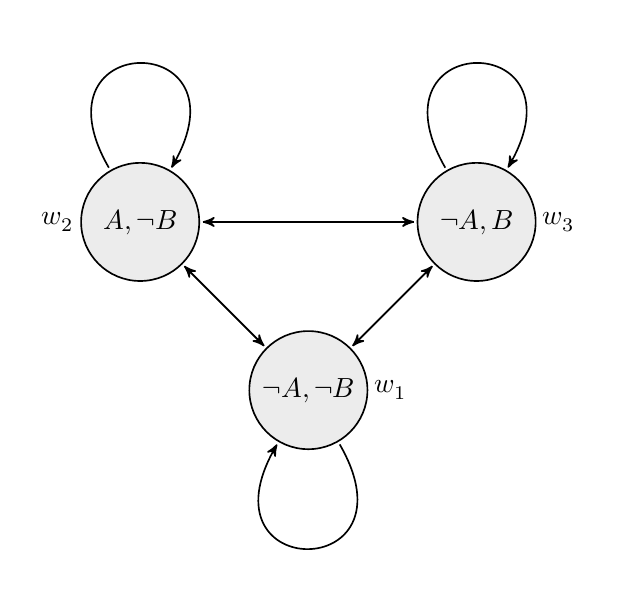
\begin{tikzpicture}[scale=0.5,modal,world/.append style={minimum size=1.5cm}]
      \node[world] (w1) [label=right:$w_1$]{$\neg A, \neg B$}; 
      \node[world] (w2) [label=left:$w_2$, above left=of w1]{$A, \neg B$}; 
      \node[world] (w3) [label=right:$w_3$, above right=of w1] {$\neg A, B$};
      \draw[->] (w1) to (w2);
      \draw[->] (w1) to (w3);
      \draw[->] (w2) to (w1);
      \draw[->] (w3) to (w1);
      \draw[->] (w3) to (w2);
      \draw[->] (w2) to (w3);
      \path[->] (w2) edge[reflexive above] (w2);
      \path[->] (w3) edge[reflexive above] (w3);
      \path[->] (w1) edge[reflexive below] (w1);
    \end{tikzpicture}
    \end{column}
    \begin{column}{0.33\textwidth}

At $w_1$, we have $\Diamond A \wedge \Diamond B$ true. 

\pause \bigskip

But nowhere is $A \wedge B$ true, so $\Diamond(A \wedge B)$ is false at $w_1$. So the conditional is false. 

\pause \bigskip

Again, this is overkill.
\end{column}
\end{columns}
\end{frame}

\begin{frame}{\(A \rightarrow \Box A\)}
\protect\hypertarget{a-rightarrow-box-a}{}
\begin{columns}
    \begin{column}{0.45\textwidth}
        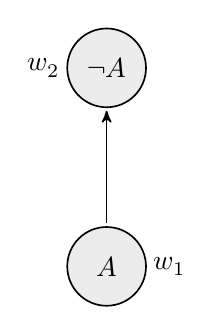
\begin{tikzpicture}[scale=0.6,modal,world/.append style={minimum size=1cm}]
      \node[world] (w1) [label=right:$w_1$]{$A$}; 
      \node[world] (w2) [label=left:$w_2$, above =of w1]{$\neg A$}; 
      \draw[->] (w1) to (w2);
    \end{tikzpicture}
    \end{column}
    \begin{column}{0.5\textwidth}
    \begin{itemize}
    \item At $w_1$ $A$ is true.
    \item But $\Box A$ is false, since $w_1$ can access $w_2$, and $A$ is false there.
    \item So $A \rightarrow \Box A$ is false.
    \end{itemize}
  \end{column}
\end{columns}
\end{frame}

\begin{frame}{\(\Box A \rightarrow A\)}
\protect\hypertarget{box-a-rightarrow-a}{}
\begin{columns}
    \begin{column}{0.45\textwidth}
        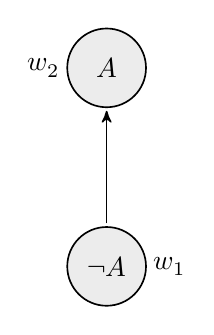
\begin{tikzpicture}[scale=0.6,modal,world/.append style={minimum size=1cm}]
      \node[world] (w1) [label=right:$w_1$]{$\neg A$}; 
      \node[world] (w2) [label=left:$w_2$, above =of w1]{$A$}; 
      \draw[->] (w1) to (w2);
    \end{tikzpicture}
    \end{column}
    \begin{column}{0.5\textwidth}
    \begin{itemize}
    \item At $w_1$ $\Box A$ is true. The only accessible world is $w_2$, and $A$ is true there.
    \item But $A$ is false there.
    \item So $\Box A \rightarrow A$ is false.
    \end{itemize}
  \end{column}
\end{columns}
\end{frame}

\begin{frame}{\(\Box \Diamond A \rightarrow B\)}
\protect\hypertarget{box-diamond-a-rightarrow-b}{}
\begin{columns}
    \begin{column}{0.45\textwidth}
        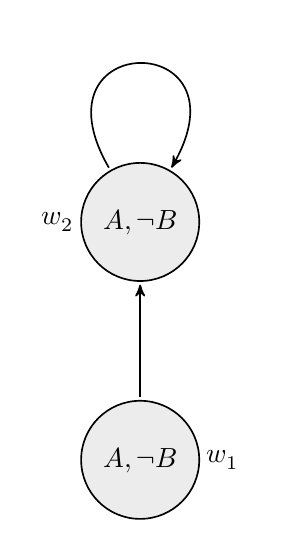
\begin{tikzpicture}[scale=0.6,modal,world/.append style={minimum size=1.5cm}]
      \node[world] (w1) [label=right:$w_1$]{$A, \neg B$}; 
      \node[world] (w2) [label=left:$w_2$, above =of w1]{$A, \neg B$}; 
      \draw[->] (w1) to (w2);
     \path[->] (w2) edge[reflexive above] (w2);
    \end{tikzpicture}
    \end{column}
    \begin{column}{0.5\textwidth}
    \begin{itemize}
    \item At $w_1$ $\Box \Diamond A$ is true. The only accessible world is $w_2$, and $\Diamond A$ is true there. (Why?)
    \item But $B$ is false at $w_1$.
    \item So $\Box \Diamond A \rightarrow B$ is false.
    \end{itemize}
  \end{column}
\end{columns}
\end{frame}

\begin{frame}{\(\Box \Diamond A \rightarrow A\)}
\protect\hypertarget{box-diamond-a-rightarrow-a}{}
\begin{columns}
    \begin{column}{0.45\textwidth}
        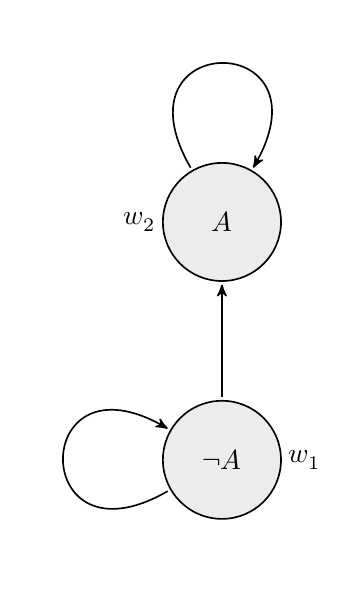
\begin{tikzpicture}[scale=0.6,modal,world/.append style={minimum size=1.5cm}]
      \node[world] (w1) [label=right:$w_1$]{$\neg A$}; 
      \node[world] (w2) [label=left:$w_2$, above =of w1]{$A$}; 
      \draw[->] (w1) to (w2);
     \path[->] (w2) edge[reflexive above] (w2);
     \path[->] (w1) edge[reflexive left] (w1);
    \end{tikzpicture}
    \end{column}
    \begin{column}{0.5\textwidth}
    \begin{itemize}
    \item At $w_1$ $\Box \Diamond A$ is true. At every world, $w_2$ is accessible, and $A$ is true there.
    \item But $A$ is false at $w_1$.
    \item So $\Box \Diamond A \rightarrow A$ is false at $w_1$.
    \end{itemize}
  \end{column}
\end{columns}
\end{frame}

\begin{frame}{\(\Box \Box A \rightarrow \Box A\)}
\protect\hypertarget{box-box-a-rightarrow-box-a}{}
\begin{columns}
    \begin{column}{0.45\textwidth}
        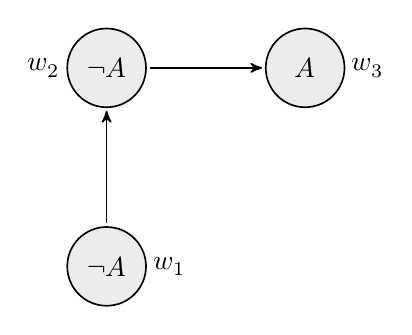
\begin{tikzpicture}[scale=0.5,modal,world/.append style={minimum size=1cm}]
      \node[world] (w1) [label=right:$w_1$]{$\neg A$}; 
      \node[world] (w2) [label=left:$w_2$, above =of w1]{$\neg A$}; 
      \node[world] (w3) [label=right:$w_3$, right =of w2]{$A$}; 
      \draw[->] (w1) to (w2);
      \draw[->] (w2) to (w3);
%     \path[->] (w2) edge[reflexive above] (w2);
%     \path[->] (w1) edge[reflexive left] (w1);
    \end{tikzpicture}
    \end{column}
    \begin{column}{0.5\textwidth}
    \begin{itemize}
    \item The only world $w_2$ can access is $w_3$, and $A$ is true there, so $\Box A$ is true at $w_2$.
    \item The only world $w_1$ can access is $w_2$, and $\Box A$ is true there, so $\Box \Box A$ is true at $w_1$.
    \item But $\Box A$ is false at $w_1$.
    \item So $\Box \Box A \rightarrow \Box A$ is false at $w_1$.
    \end{itemize}
  \end{column}
\end{columns}
\end{frame}

\begin{frame}{\(\Box A \rightarrow \Box \Box A\)}
\protect\hypertarget{box-a-rightarrow-box-box-a}{}
\begin{columns}
    \begin{column}{0.45\textwidth}
        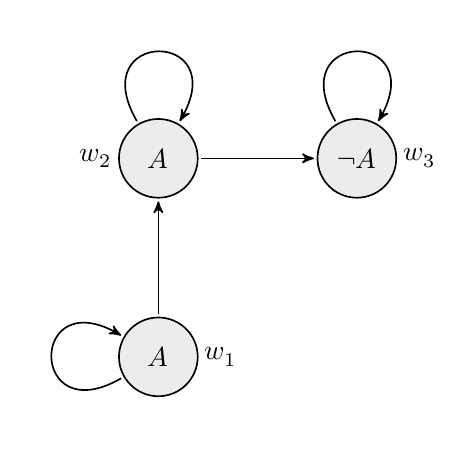
\begin{tikzpicture}[scale=0.5,modal,world/.append style={minimum size=1cm}]
      \node[world] (w1) [label=right:$w_1$]{$A$}; 
      \node[world] (w2) [label=left:$w_2$, above =of w1]{$A$}; 
      \node[world] (w3) [label=right:$w_3$, right =of w2]{$\neg A$}; 
      \draw[->] (w1) to (w2);
      \draw[->] (w2) to (w3);
     \path[->] (w2) edge[reflexive above] (w2);
     \path[->] (w3) edge[reflexive above] (w3);
     \path[->] (w1) edge[reflexive left] (w1);
    \end{tikzpicture}
    \end{column}
    \begin{column}{0.5\textwidth}
    \begin{itemize}
    \item Since $A$ is false at $w_3$, and $w_2$ can access $w_3$, $\Box A$ is false at $w_2$.
    \item Since $\Box A$ is false at $w_2$, and $w_1$ can access $w_2$, $\Box \Box A$ is false at $w_1$.
    \item But $\Box A$ is true at $w_1$.
    \item So $\Box A \rightarrow \Box \Box A$ is false at $w_1$.
    \end{itemize}
       \end{column}
\end{columns}
\end{frame}

\begin{frame}{\(\Box A \rightarrow \Diamond A\)}
\protect\hypertarget{box-a-rightarrow-diamond-a}{}
\begin{columns}
    \begin{column}{0.45\textwidth}
        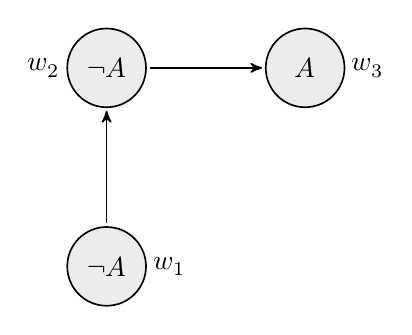
\begin{tikzpicture}[scale=0.5,modal,world/.append style={minimum size=1cm}]
      \node[world] (w1) [label=right:$w_1$]{$\neg A$}; 
      \node[world] (w2) [label=left:$w_2$, above =of w1]{$\neg A$}; 
      \node[world] (w3) [label=right:$w_3$, right =of w2]{$A$}; 
      \draw[->] (w1) to (w2);
      \draw[->] (w2) to (w3);
%     \path[->] (w2) edge[reflexive above] (w2);
%     \path[->] (w1) edge[reflexive left] (w1);
    \end{tikzpicture}
    \end{column}
    \begin{column}{0.5\textwidth}
    \begin{itemize}
    \item Focus on $w_3$.
    \item There is no accessible world where $A$ is false, so $\Box A$ is true there.
    \item But there is no accessible world where $A$ is true, so $\Diamond A$ is false there.
    \item So $\Box A \rightarrow \Diamond A$ is false there.
    \end{itemize}
\end{column}
\end{columns}
\end{frame}

\begin{frame}{\(\Box A \rightarrow \Diamond A\)}
\protect\hypertarget{box-a-rightarrow-diamond-a-1}{}
\begin{columns}
    \begin{column}{0.45\textwidth}
        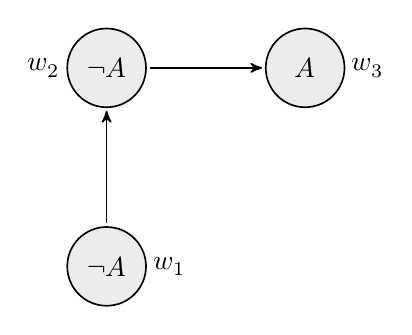
\begin{tikzpicture}[scale=0.5,modal,world/.append style={minimum size=1cm}]
      \node[world] (w1) [label=right:$w_1$]{$\neg A$}; 
      \node[world] (w2) [label=left:$w_2$, above =of w1]{$\neg A$}; 
      \node[world] (w3) [label=right:$w_3$, right =of w2]{$A$}; 
      \draw[->] (w1) to (w2);
      \draw[->] (w2) to (w3);
%     \path[->] (w2) edge[reflexive above] (w2);
%     \path[->] (w1) edge[reflexive left] (w1);
    \end{tikzpicture}
    \end{column}
    \begin{column}{0.5\textwidth}
    Whenever there are no accessible worlds, the following two weird things happen.
    \begin{enumerate}
    \item All $\Box$-sentences (i.e., sentences that start with a $\Box$ that takes scope over the whole sentence) are true.
    \item All $\Diamond$-sentences (i.e., sentences that start with a $\Diamond$ that takes scope over the whole sentence) are false.
    \end{enumerate}
   \end{column}
\end{columns}
\end{frame}

\begin{frame}{For Next Time}
\protect\hypertarget{for-next-time}{}
We will start looking at frames - what you get when you remove the
valuation from a model.
\end{frame}

\end{document}
